\chapter{引言}
\section{研究背景}
% 介绍图计算

%图计算很有用
图(Graph)是一种重要的数据结构,它由顶点与边构成。
如图\ref{fig:graph_important}所示,
图能够对很多问题进行抽象建模,
图计算在很多领域发挥了重要的作用。
比如在facebook、twitter、weibo这些社交网络中,用户可以被看作顶点,
用户之间建立的关系可以被看作边,这样社交网络中的各种规律就能用图来研究。
在互联网中通过把web网页看作顶点,
把页面之间的超链接看作边,人们就可以通过图来研究网页的权重排名信息。
而随着大数据时代的到来,如何对海量图数据进行高效的分析处理愈加成为工业和学术界的研究热点。

% 图(Graph)是一种重要的数据结构,它由顶点与边构成。
% 利用这种数据结构,我们能够对社交网络计算、广告、网页数据挖掘等各个方面进行抽象建模,从而获得有用信息(图\ref{fig:graph_important})。
% 在facebook、twitter、weibo这些社交网络中,我们可以把用户看作顶点,
% 把用户之间建立的关系看作边,从而进行社交网络中各种规律的研究。
% 在互联网中,我们通过把web网页看作顶点,
% 把页面之间的超链接看作边,利用这些信息研究网页的权重排名。
% 而随着大数据时代的到来,如何对海量图数据进行高效的分析处理愈加成为工业和学术界的研究热点。
\begin{figure}[!htbp]
  \centering
  
\includegraphics[width=0.40\textwidth]{graphs_are_everywhere.png}
  \bicaption{图计算的应用领域}{Application areas of graph computing}
  \label{fig:graph_important}
\end{figure}

%人们开发了很多框架进行图计算
传统的大数据处理平台使用MapReduce\cite{mapreduce}这种函数式编程范式,但这种编程范式并不适用于图计算。
基于函数式编程思想的MapReduce需要在每次迭代之间传递数据,
而图计算由于结构的内在复杂性,计算往往是不规则的,只有部分图数据参与计算,
那些不参与计算的数据在处理过程不需要传递。
此外图算法若要用MapReduce实现往往需要转换为一系列MapReduce任务,这又会带来额外的存储读写开销,
所以传统的大数据处理平台无法胜任大规模图计算任务\cite{Malewicz@SIGMOD10}。
为此人们开发了许多专门用于处理大规模图数据的分布式并行计算框架。    
\cite{Malewicz@SIGMOD10, Low@12, Gonzalez@OSDI12, Zhu@OSDI16, Gonzalez@OSDI14, Avery@HS11, Shao@SIGMOD13, 
Chen@EuroSys15, Xie@PPoPP15, Roy@SOSP15, Seo@CloudCom10, Gregor@POOSC15, Hoque@TRIOS13, Teixeira@SOSP15}

\section{针对副本点的延迟数据一致性方法}

%介绍副本点
当大规模图数据在集群中划分存储时,图中的顶点就出现了副本点。副本点在现有的分布式图计算编程框架中充当着关键角色。
它使得框架可以对单个顶点进行并行处理,并使不同机器上的邻居顶点在本地互相访问数据成为可能。
然而副本点在带来巨大好处的同时也引入了数据一致性(data coherency)的问题。\cite{Wang@PPoPP18, zlj2018}
分布式图计算编程框架要维护不同机器上存储的副本点$v_1, v_2, \cdots, v_k$之间的数据一致性。
% 这些图计算框架都要把大规模图数据在集群中分布式存储,因此副本点在现有的分布式图计算编程框架中充当着关键角色。  
% 副本点使得集群中的多台机器可以对一个顶点$v$并行地计算,同时也使得每个顶点可以在本地访问远程顶点,减少了机器之间的通讯开销。 

图\ref{fig:mirror}展示了一个小图在4台机器上划分后的结果,可以看到中心的顶点产生了4个副本点。
当4台机器并行计算改变顶点上的数据时,图计算要框架要负责维护这4个副本点之间的数据一致。

\begin{figure}[!htbp]
  \centering
  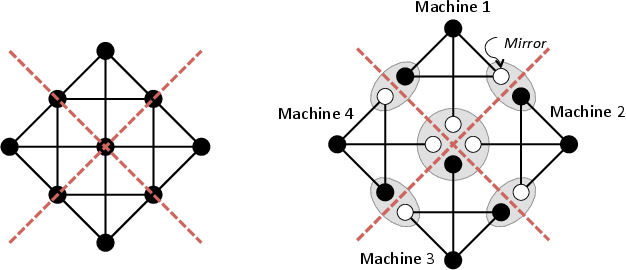
\includegraphics[width=0.40\textwidth]{mirror}
  \bicaption{副本点示意图}{schematic diagram of mirror vertex}
  \label{fig:mirror}
\end{figure}

%副本点存在的问题

很多编程框架都把每个顶点看做一个原子性的点,使用 急切数据一致性(eager data coherency )方法来保证所有副本之间的数据是一致的,
每个点横跨的机器数量和数据同步频率直接影响系统通信量的大小进而影响系统的性能。
在这种方法中,系统把顶点$v$的副本点中的其中一个标记为master点,其他副本点为mirror点,其中master点保存了该顶点的真实数据,
而mirror点只实时地保存着master点数据的一份本地拷贝。
对顶点$v$的所有更新必须在master点上进行,更新完成后都会立即通过消息传递把最新状态发送给所有副本,这带来了频繁的全局同步和消息通信。

%lazygraph 的解决思路
对于一些经典的图算法某个点的解往往只依赖于它部分的邻居顶点,
而对于数据挖掘和机器学习类的图算法中间过程的不一致往往不会影响最终的收敛性。
对于绝大多数图算法,系统时刻维护副本点之间的数据一致并不是必须的。
基于这些观察,针对 eager data coherency 存在的问题,
我们在之前的工作\cite{Wang@PPoPP18}中提出了一种延迟数据一致性方法(LazyAsync)\cite{zlj2018},
它基于延迟数据一致性(lazy data coherency)的思想,有效地降低了系统由维护副本点之间数据一致所引起的开销。

在LazyAsync中,顶点的不同副本点被看作互相独立的点,各自迭代更新,最后通过计算实现数据一致。
LazyAsync要求图算法的迭代的公式写为差值累加的形式,
顶点的各副本点只在全局消息处理时交换差值消息,
顶点计算过程中不产生的数据同步和消息交换。
基于 lazy data coherency 的思想,
顶点的多个副本点各自独立地进行数轮本地计算后会交换本地差值消息累加和,
由于积累了同样的消息累加和,各副本之间通过计算实现了数据一致。

%lazygraph 的效果
由于单个迭代计算过程中副本点之间不必同步,多轮迭代计算过程之间副本点之间延迟同步,
系统极大地减少了全局数据同步和通信的开销。
我们在具有代表性的分布式并行图计算框架PowerGraph\cite{Gonzalez@OSDI12}上实现了LazyAsync 这种方法。
在48个虚拟机的EC2的集群环境下的实验结果表明,在4种典型的图算法和不同种类的真实输入图上,
LazyAsync 在保证正确性的基础上,相较于PowerGraph原始基于 eager data coherency 的同步引擎方法
获得了1.25倍到10.69倍的加速比。


\section{延迟数据一致性方法尚未解决的问题}
% lazygraph 的性能提升效果依赖于具体的延迟一致开启策略
% lazygraph 现在采用一个决策树模型作为开启策略,它存在着以下这些方面的不足
% 1. 难以解释
% 2. 训练过程依赖于手动调优
% 3. 无法做到自适应
虽然我们提出的LazyAsync极大地提升了分布式图计算的性能,但是它在以下几个方面还存在着一系列尚未解决的问题。    
\begin{enumerate}      
  \item[(一)] LazyAsync 的开启策略和系统最终得到的性能提升程度的关系有待研究 \newline\indent
    LazyAsync 的开启策略指的是系统应该在何时对副本点开启 lazy data coherency,
    让各副本点独立计算数轮之后再进行消息交换。
    一种策略是立即进入策略,即系统一开始运行就启用 lazy data coherency。
    另一种策略是手动调优策略,即不断的手动指定启用 lazy data coherency 的全局超步迭代轮次,
    然后取其中性能提升最好的一个结果。
    手动调优策略虽然不实用但是能够得出LazyAsync在指定算法和输入图上的相对最优的性能提升效果。
    在实验中我们发现,随着这些具体策略的不同,系统得到的加速比也不同。
    在有些算法和输入图上立即进入策略就能得到相对最好的性能提升效果,
    在有些算法和输入图上需要手动调优才能得到相对最好的性能提升效果。
    在不同的算法和输入图上,开启策略如何影响系统最后拿到的性能提升这一问题尚未研究清楚。

  \item[(二)] 目前系统实现的决策树方法存在缺陷 \newline\indent
    虽然开启策略如何影响性能提升这一问题尚未研究清楚,
    但我们基于手动调优的数据实现了一种决策树方法来作为开启策略。
    % LazyAsync 需要结合具体的应用算法和输入图选择合适的时间节点进行数据一致。
    这种决策树方法通过离线训练的方式得到,
    它依赖于对各种算法和输入图组合手动调优所产生的数据集,耗费时间较长,
    并且对于新的算法和输入图组合不能保证得到相对最优的性能提升,
    这对于一个实用的图计算系统来说是不可接受的。
    % 因此我们需要对目前的系统实现进行改进,把这个过程自动化,使得系统的模型具有足够的泛化能力,能够自适应的处理各种输入。          

  \item[(三)] 目前的系统缺乏一个考虑各种影响因素的自适应优化策略 \newline\indent
    %how to say?
    虽然我们提出了一种行之有效,且证明正确的延迟数据一致性方法(LazyAsync),
    但是这个方法目前还缺乏一个自适应各种影响因素的优化策略。
    对于采用了 LazyAsync 的分布式并行图计算系统,开启策略,具体的算法用例,
    输入图结构特征,图划分算法,配置环境等都会对最终的性能造成影响,
    并且在系统执行过程中这些因素是动态变化而又互相影响的,
    为了得到相对最优的性能提升效率,系统需要一个能够自适应这些外部因素变化的优化策略,实时监控这些因素动态地调节全局同步的频率。          
    % 以及目前的系统实现中只在同步引擎上实现了LazyAsync,而有些算法更适合异步引擎,因此这种方法是否能够应用到异步引擎中也有待研究。
\end{enumerate}
\section{基于解的局部性的自适应优化方法}
% 通过实验发现, 解存在着局部性规律可以作为自适应开启策略
为了解决LazyAsync目前存在的问题,本研究首先对这种方法的性能收益波动现象进行了分析。
在之前的工作中,我们从分布式计算系统的角度解释了LazyAsync的性能收益的来源。
LazyAsync减少了图计算的超步迭代次数,极大地降低了系统的全局同步等待和集群之间的通信这些开销,
从而得到了性能提升。
但是这种阐述只能说明LazyAsync方法能够提升性能这个定性的问题,
却无法解释LazyAsync性能收益波动的问题。
并且在实际的实验中我们发现,在某些情况下LazyAsync虽然减少了迭代次数,但是最终却并没有拿到计算时间上的性能收益。

通过定义有效计算的概念,本研究最终找到了LazyAsync的性能收益波动现象背后的原因。
本研究发现LazyAsync虽然避免了eager data coherency 方法中存在的冗余的同步,等待和通信,
但是却有可能在本地计算中引入新的冗余计算。
在LazyAsync不同的开启策略中,那些性能提升更好的情况是因为进行了更多的有效计算,
而那些性能提升相对不好的情况则是因为进行了更多的冗余计算。
所以,LazyAsync要想得到相对最优的性能提升,就要从提高有效计算的比例入手。


通过分析,本研究发现LazyAsync能否进行更多的有效计算和顶点上的全局解和局部解的关系规律有关。
在分布式图计算中,由于副本点的存在,每个顶点上的全局解由多个局部解构成。
LazyAsync在数据一致性阶段通过交换构成局部解的消息累加值来然后进行计算来实现不同副本点上的全局解的一致。
而在数据一致性阶段之间,各个副本点上在本地进行不需要消息交换和通信的本地计算。
这些本地计算能维持较高的有效计算的比例时,LazyAsync就能获得较高的性能收益。

另一方面,当顶点上的全局解只由一个局部解构成时,本地计算就能进行更多的有效计算,
当顶点上的全局解由多个局部解构成时,本地计算就容易造成更多的无效计算。
在图计算过程中,全局解由单个局部解构成和由多个局部解构成的情况都是同时存在的。
如果大部分活跃点的全局解只由单个局部解构成,那么此时开启lazy data coherency 
LazyAsync就能够通过多轮的本地计算对本地子图进行事先的有效计算,减少冗余计算,
最终得到较好的性能提升,
对于这种情况,本研究称之为解的局部性。
本研究通过统计迭代过程中由单个局部解构成全局解这样具有解的局部性规律的活跃点的比例来
判断图计算整体解的局部性的变化规律。



全局解和局部解的关系影响着LazyAsync的有效计算的程度,进而影响了这种方法的性能提升相对大小。
经过一系列实验之后,本研究进一步找到了全局解和局部解的关系变化规律。
本研究发现,在图计算过程中,随着计算的进行,全局解由多个局部解构成的点的数量会逐渐下降,
并且在每轮的活跃点中只占一小部分比例。
也就是说,随着计算的进行,图计算中的大部分顶点的全局解只由某一个局部解构成。
图计算整体表现出明显的解的局部性。
正是由于解的局部性的存在,LazyAsync才能通过lazy data coherency 来减少系统中的数据交换从而获得性能收益。


\begin{figure}[!htbp]
  \centering
  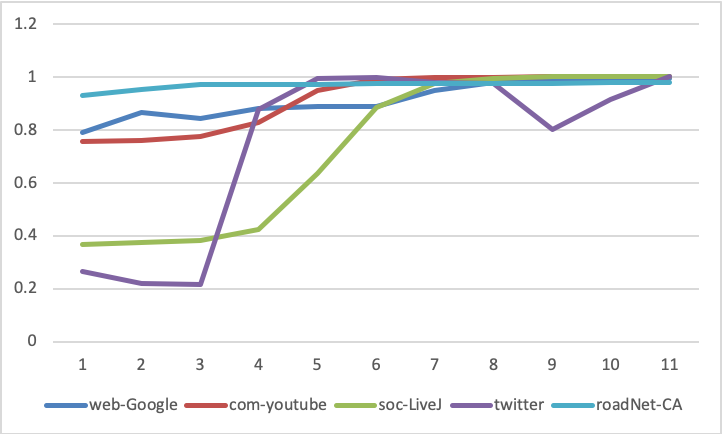
\includegraphics[width=0.40\textwidth]{ch1percent}
  \bicaption{不同输入图上解的局部性的活跃点的比例变化}
  { Proportion of active vertices with localization of solutions on different input graphs}
  \label{fig:ch1percent}
\end{figure}

然而解的局部性并不是一直存在的,这也是LazyAsync需要合适的开启策略的重要原因。
通过实验本研究发现,解的局部性和具体的输入图和算法用例以及集群的配置有关。
随着这些外部输入条件的不同,解的局部性也有着不同的变化规律。
图\ref{fig:ch1percent}给出的Connected Component(CC)算法在5个不同的输入图上的一个实验结果
可以直观地说明这一点。
这个图中统计了迭代过程中由单个局部解构成全局解这样具有解的局部性规律的活跃点的比例的变化趋势,
图中横坐标代表全局超步的迭代轮次,纵坐标代表此轮超步迭代中解的局部性的活跃点的比例。
在有的图上,一开始就一直呈现出较为明显的解的局部性的规律,即全局解由多个局部解构成的顶点一直只占极少一部分。
而在另外一些图上,一开始解的局部性现象并不存在,而是存在着全局解由多个局部解构成的顶点数量一直在增长的过程。
当这样的顶点数量在增长时,是不适宜开启lazy data coherency 的。

在之前的工作中,我们通过机器学习的手段找到了一个决策树模型作为开启策略。
这个决策树使用输入图的边点比例和运行时的活跃点变化趋势作为开启策略的判断条件。
通过实验本研究发现,决策树所使用的特征其实也是对解的局部性变化规律的间接反映。
% 同时,由于决策树是对手动调优产生的训练集的数据拟合

最终,通过在运行时动态的监控全局解由多个局部解构成的顶点的数量和比例,本研究得到了一个基于解的局部性的自适应优化方法。
这个自适应优化方法在动态观察到图计算迭代过程中开始存在解的局部性时,就开启lazy data coherency。
这种方法克服了之前的决策树模型存在的失灵问题,同时也不需要事先的手动调优产生数据集来进行训练。
此外,由于解的局部性是受输入图特性,算法用例,集群配置环境所共同影响的,所以这种方法能够实现对这些不同外部输入条件的自适应。

总而言之,本研究的主要创新点和贡献可以归纳为以下几点:

1. 对LazyAsync的在不同开启策略下得到不同性能提升这一现象进行了研究,认清了这一方法的性能提升规律。
以具体的例子识别出了LazyAsync虽然避免了eager data coherency 方法存在的冗余同步和通信,但是引入了新的冗余计算。
并且正是这种冗余计算造成了LazyAsync在不同开启策略性下得到不同程度的性能提升。

2. 对图计算过程中活跃点上全局解和局部解之间的关系进行了研究,发现了解的局部性这一现象。
通过分析,本研究发现随着图计算的进行,每次迭代中大部分活跃点的全局解只由某个局部解构成,
那么此时局部解所在的副本点完全不需要等待和同步其他副本点就可以继续进行图计算过程。
而这种情况正是LazyAsync有利于减少冗余计算,有利于开启lazy data coherency的情况。

3. 基于解的局部性这一现象,设计并实现了基于解的局部性的自适应优化方法。
这种方法解决了LazyAsync在不同的输入条件下如何得到相对最优的性能提升这一问题。
相较于之前采用的决策树方法,这种方法不需要事先的离线调优和训练,更不存在某些输入条件下失灵的问题。


%从 到 最终 我们发现了。。。


\section{全文结构}
% 每一章写了什么
本文各章节的具体内容安排如下:

第一章是引言。介绍了我们之前针对分布式并行图计算框架中副本点存在的问题所提出的LazyAsync这一研究背景。
然后介绍了这个方法所遗留的问题,以及本研究针对这些问题所做的工作。

第二章是相关工作介绍。介绍了分布式图计算中主要的研究主题,并对本研究所采用的分布式图计算系统LazyGraph做了重点介绍。
在对LazyGraph的介绍中尤其详细地介绍了LazyAsync和它的开启策略问题。
本研究正是在这些工作的基础上进一步展开的。

第三章LazyAsync性能收益波动现象分析。
首先对LazyAsync的性能收益的来源进行了研究。
从具体算法的角度,本研究展示了这种方法的性能收益来自于 它能够在本地计算所进行的额外多轮迭代中提前激活顶点并使之收敛。
然后通过分析具体的例子,本研究提出在这种本地计算中存在着冗余无效的计算,并且这些冗余计算会造成性能损失。
最后本研究通过具体的实验验证了这一观点。
从lazy data coherency 带来的性能收益,到冗余计算带来的性能损失,本研究在这一章发现
本地计算中存在着不同程度的冗余计算
造成了
LazyAsync不同开启策略下得到不同程度的性能提升这一
性能收益波动的现象。

第四章基于解的局部性的自适应优化方法。
冗余计算影响影响收益,
本章先是介绍了全局解和局部解的关系如何影响冗余计算。
然后通过离线分析的方法,本章对不同算法和输入图上全局解和局部解之间的关系进行了实验分析,
发现了全局解和局部解之间存在着局部性规律。
接下来通过在线统计的方法,本章提出了基于解的局部性的自适应优化方法用于指导LazyAsync的开启策略。
最后,本章在不同算法和输入图上进行了实验评测,并对评测结果进行了分析。

最后一章对全文的研究内容进行了总结和展望。




